\chapter{Results}
\section{Naive fitted method}
\begin{figure}[H]
\centering
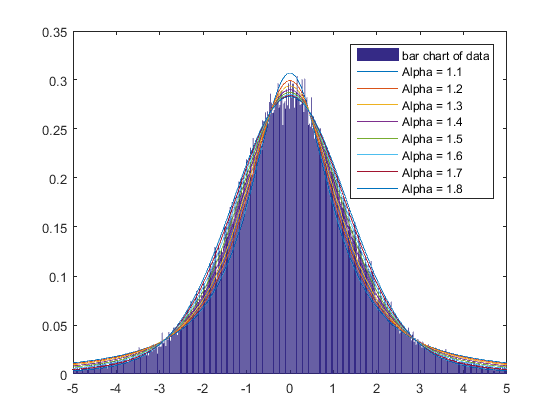
\includegraphics[width=1\textwidth]{billeder/alpha1_6_naivefit}
\caption{Fitted distributions and histogram with $\alpha = 1.6$}
\label{fig:naivefitres}
\end{figure}
The output from the method is:\\
Most Likely Alpha value is\\
Alpha = 1.6\\

\section{log|S$\alpha$S| method}
\begin{figure}[H]
    \centering
    \begin{minipage}{.5\textwidth}
        \centering
        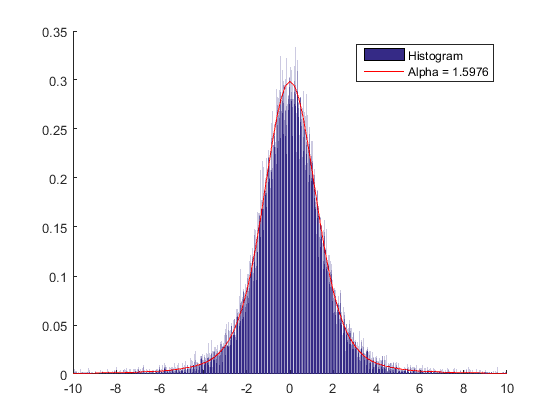
\includegraphics[width=1\textwidth]{billeder/alpha1_6_logsas}
		\caption{Estimated distribution and histogram with $\alpha = 1.6$}
		\label{fig:logsas16}
    \end{minipage}%
    \begin{minipage}{0.5\textwidth}
        \centering
        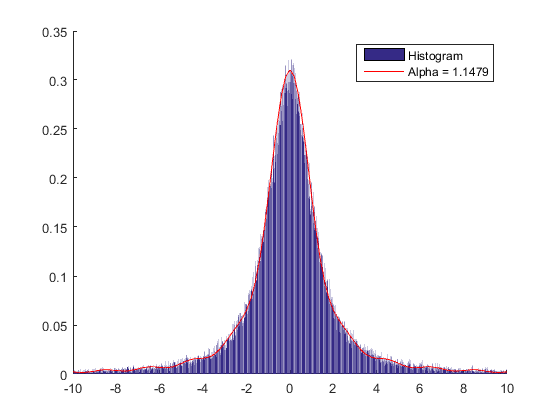
\includegraphics[width=1\textwidth]{billeder/alpha1_15_logsas}
		\caption{Estimated distribution and histogram with $\alpha = 1.15$}
		\label{fig:logsas115}
    \end{minipage}
\end{figure}

\begin{table}[H]
	\center
    \begin{tabular}{|l|l|l|}
    \hline
    True Alpha & Estimated Alpha & \% Error \\ \hline
    1          & 0.9984          & 0.16     \\ \hline
    1.15       & 1.1479          & 0.18     \\ \hline
    1.3        & 1.2975          & 0.19     \\ \hline
    1.45       & 1.4473          & 0.19     \\ \hline
    1.6        & 1.5976          & 0.15     \\ \hline
    \end{tabular}
    \caption{True and estimated alpha values for log|S$\alpha$S| method}
    \label{tab:resalpha}
\end{table}